\documentclass{emulateapj}
%\documentclass[12pt,preprint]{aastex}

\usepackage{hyperref}

\usepackage{graphicx}
\usepackage{float}
\usepackage{amsmath}
\usepackage{epsfig,floatflt}
\usepackage{listings}
\usepackage{gensymb}
\usepackage{upgreek}
\usepackage{csquotes}
\usepackage{color}
% \usepackage{natbib}


\lstset{frame=tb,
  language=Python,
  aboveskip=3mm,
  belowskip=3mm,
  showstringspaces=false,
  columns=flexible,
  basicstyle={\small\ttfamily},
  numbers=none,
  numberstyle=\tiny\color{gray},
  keywordstyle=\color{blue},
  commentstyle=\color{dkgreen},
  stringstyle=\color{mauve},
  breaklines=true,
  breakatwhitespace=true,
  tabsize=3
}

\newcommand\p[2]{\frac{\partial #1}{\partial #2}}
\newcommand\Lag[1]{\frac{d}{dt}\left( \dfrac{\partial L}{\partial \Dot{#1}}\right) - \dfrac{\partial L}{\partial #1} &= 0}


\begin{document}

\title{Computational Physics - Project 1}

\author{
  Dahl, Jon Kristian \\
  \and
  Sand, Mats Ola \\
  \and
  Fløisand, Johan Andreas \\
}

\begin{abstract}
Many problems in physics stems from solving differential equations. For a few number of systems, these equations are exactly solvable, but for many more, analytical solutions does not exist. We look at how a simple differential equation (Poisson's equation) can be discretized into a linear algebra problem, and look at how three different algorithms solve it. We use the Thomas algorithm, a specialized Thomas algorithm and LU decomposition followed by Gaussian elimination. We find that for our second order differential equation, the specialized Thomas outperforms the other algorithms since it uses $4n$ floating point operations, compared to the $9n$ and $2/3n^3$ for the Thomas algorithm and LU decomposition respectively. For error analysis we find that the Thomas algorithm and the specialized Thomas algorithm are equal and has a max relative error as low as $10^{-9}$, but the LU solution gives weirdly bad results at small grid point values, $n$.
\end{abstract}

%%%%%%%%%%%%%%%%%%%%%%%%%%%%%%%%%%%%
%%%%%%%%%%%%%%%%%%%%%%%%%%%%%%%%%%%%
\section{Introduction}
%%%%%%%%%%%%%%%%%%%%%%%%%%%%%%%%%%%%
%%%%%%%%%%%%%%%%%%%%%%%%%%%%%%%%%%%%
    Linear algebra naturally occurs in computational physics due to problems where continuous parameters needs to be discretized. Natural examples of this are differential equations which are not analytically solvable that needs to be solved numerically. In this report we will solve Poisson's equation \cite[Chapter 13]{matmet}, \(-\frac{d^2u}{dx^2} = f(x)\), by discretizing it into a linear algebra problem which can be solved by a simple matrix equation. We will solve the matrix equation using three different algorithms and then compare the relative numerical error and computation time between each of them.
    
    The three algorithms are: The Thomas algorithm for a general tridiagonal matrix, a Thomas algorithm specially designed for the matrix representing Poisson's equation (i.e., a tridiagonal T\"{o}plitz matrix), and lastly LU decomposition for a dense matrix.
    \newline
    \newline
    We begin with a method section where we introduce the differential equation and explain the algorithms. The results section follows where we compare the relative errors and computation times of the algorithms. Finally, we discuss our results and conclude how each algorithm fits different purposes.
    
    All program code is supplied in a GitHub repository: \url{https://github.com/johanafl/FYS3150-4150/tree/master/project1}.

%%%%%%%%%%%%%%%%%%%%%%%%%%%%%%%%%%%%
%%%%%%%%%%%%%%%%%%%%%%%%%%%%%%%%%%%%
\section{Method}
%%%%%%%%%%%%%%%%%%%%%%%%%%%%%%%%%%%%
%%%%%%%%%%%%%%%%%%%%%%%%%%%%%%%%%%%%
    Lets now introduce Poisson's equation and show how we can find an expression for the double derivative of a function using Taylor series \cite[Chapter 11]{kalkulus}.
    %We introduce the Poisson equation and show how we can find an expression for the double derivative of a function using Taylor series. We show how this can be discretized into a single tridiagonal matrix equation which can be solved by the Thomas algorithm. Since the matrix is a T\"{o}plitz matrix
    %Finally we show that we can also use the standard LU decomposition and .
    %%%%%%%%%%%%%%%%%%%%%%%%%%%%%%%%%%%%
    \subsection{Poisson's equation}
    %%%%%%%%%%%%%%%%%%%%%%%%%%%%%%%%%%%%
        Poisson's equation \cite[Chapter 13]{matmet} pops up in several problems in physics, for instance in the electrostatic potential \(\Phi\):
        
        \begin{equation*}
            \nabla^2\Phi = -4\pi\rho(\mathbf{r}).
        \end{equation*}
        Assuming that the electrostatic potential only depends on the radial distance \(r\), a few lines of algebra shows that we get back Poisson's equation, \(\frac{d^{2}\phi(r)}{dr^{2}}=-4\pi r\rho(r)\). Rewriting \(\phi\rightarrow u\) and \(r\rightarrow x\) we are left with:
        
        \begin{equation}\label{eq:Poisson_equation}
            -\frac{d^{2}u(x)}{dx^{2}} = g(x).
        \end{equation}
        This is the form of the equation we will work with.
        
        In this report we will look at how three different algorithms perform when solving Poisson's equation. To see how the errors of the different algorithms unfold, we can choose \(g\) such that an exact solution for \(u\) exists. We apply our function \( u \) on the interval \([0,1]\) with the Dirichlet boundary conditions \cite[Chapter 13]{matmet}, which we set to be \(u(0) = u(1) = 0\). Choosing
        
        \begin{equation*}
            g(x) = 100e^{-10x},
        \end{equation*}
        which has the exact solution
        
        \begin{equation*}
            u(x) = 1 - \left(1 - e^{-10}\right)x - e^{-10x},
        \end{equation*}
        for the given boundary conditions, the analytical error can be computed as we will see in the next section. To see that this is the exact solution we plug it back into Poisson's equation:
        
        \begin{align*}
            -\frac{d^{2}u(x)}{dx^{2}} &= 
            \frac{d^{2}}{dx^{2}}(-1) + \frac{d^{2}}{dx^{2}}\left(1 - e^{-10}\right)x + \frac{d^{2}}{dx^{2}}e^{-10x} \\
            &= \frac{d}{dx}\left(1 - e^{-10}\right)+  \left(-10\right)^{2}e^{-10x} \\
            &= 100e^{-10x} = g(x).
        \end{align*}
        We also have 
        
        \begin{align*}
            u(0) &= 1 - \left(1 - e^{-10}\right)\cdot0 - e^{-10\cdot0} 
            = 1 - e^{0} = 0 \\
            u(1) &= 1 - \left(1 - e^{-10}\right)\cdot1 - e^{-10\cdot1} 
            = e^{-10} - e^{-10} = 0 
        \end{align*}
    %%%%%%%%%%%%%%%%%%%%%%%%%%%%%%%%%%%%
    \subsection{Approximation of the second derivative}
    %%%%%%%%%%%%%%%%%%%%%%%%%%%%%%%%%%%%
        The Taylor series of a function \(f\) about the point \(a\) is given by (see \cite[Chapter 11]{kalkulus})
        
        \begin{equation*}
            f(x) = \sum_{n=0}^{\infty}\frac{1}{n!}\left(x-a\right)^{n}f^{(n)}(a),
        \end{equation*}
        where we define \(f^{(n)}(a)\) for \(n\in\mathbb{N}\cup\{0\}\) as the \(n\)th derivative of \(f\) evaluated at \(a\). Using \textquote{Big O} notation, we write the series as
        
        \begin{equation*}
            f(x) = \sum_{n=0}^{k}\frac{1}{n!}\left(x-a\right)^{n}f^{(n)}(a) + \mathcal{O}\big((x-a)^{k}\big),
        \end{equation*}
        where \(\mathcal{O}\big((x-a)^{k}\big)\) contains the rest of the series. To see the exact form of the rest, see \cite[Chapter 11]{kalkulus} and \cite[Chapter 9]{matinf}. Assuming that the value \(x\) is fairly close to \(a\), the leading term of the rest will go as \((x-a)^{k}\). Thus, we can approximate the series as 
        
        \begin{equation*}
            f(x) \approx \sum_{n=0}^{k}\frac{1}{n!}\left(x-a\right)^{n}f^{(n)}(a),
        \end{equation*}
        with an error of order \(\mathcal{O}\big((x-a)^{k}\big)\).
        
        If we now chose \(x = x + h\) and \(a = h\), we find
        
        \begin{equation*}
            f(x+h) = f(x) + hf^{\prime}(x) + \frac{1}{2!}h^{2}f^{\prime\prime}(x) + \frac{1}{3!}h^{3}f^{\prime\prime\prime}(x) + \mathcal{O}_{1}\big(h^{4}\big).
        \end{equation*}
        For \(x = x - h\) and \(a = h\), we have
        
        \begin{equation*}
            f(x-h) = f(x) - hf^{\prime}(x) + \frac{1}{2!}h^{2}f^{\prime\prime}(x) - \frac{1}{3!}h^{3}f^{\prime\prime\prime}(x) + \mathcal{O}_{2}\big(h^{4}\big).
        \end{equation*}
        Adding the two equation gives
        
        \begin{equation*}
            f(x+h) + f(x-h) = 2f(x) + h^{2}f^{\prime\prime}(x) + \overbrace{\mathcal{O}_{1}\big(h^{4}\big) + \mathcal{O}_{2}\big(h^{4}\big)}^{\mathcal{O}\big(h^{4}\big)}.
        \end{equation*}
        Solving for the double derivative we have
        
        \begin{equation*}%\label{eq:f_double_derivative_taylor}
            f^{\prime\prime}(x) = \frac{f(x+h) - 2f(x)+ f(x-h)}{h^{2}} + \mathcal{O}\big(h^{2}\big).
        \end{equation*}
        %\newline
        %\newline
        %\newline
        %where we define \(f^{n}\) for \(n\in\mathbb{N}\cup\{0\}\) as the composition of \(f\) with itself \(n\) times. That is 
        %\begin{equation*}
        %    f^{n}(x) = \overbrace{(f\circ f\circ\ldots\circ f)}^{n\text{ times}}(x) = \overbrace{f(f(\ldots(f}^{n\text{ times}}(x))\ldots))
        %\end{equation*}
    
    %%%%%%%%%%%%%%%%%%%%%%%%%%%%%%%%%%%%
    \subsection{Discretizing and setting up a matrix equation}
    %%%%%%%%%%%%%%%%%%%%%%%%%%%%%%%%%%%%
        Our function can not be represented continuously on a computer. Hence we need to discretize the problem. To see how we can do this we will choose to discretize the interval \([0,1]\) with a finite number of discrete points \(n\). If we choose linearly spaced points we will have a step size \(h = \frac{0 - 1}{n}\) and we define 
        \begin{align*}
            &f_{0}=f(0\cdot h),\quad f_{1}=f(1\cdot h),\quad f_{2}=f(2\cdot h),\quad \ldots,\\ &f_{i}=f(i\cdot h),\,\ldots,\, f_{n-1}=f((n-1)\cdot h),\quad f_{n}=f(n\cdot h).
        \end{align*}
        We recognize $u^{\prime\prime}$ by its Taylor series and Poisson's equation (\ref{eq:Poisson_equation}) thus becomes
        \begin{equation}\label{eq:f_double_derivative_taylor}
            \frac{-u(x+h) + 2f(x) - f(x-h)}{h^{2}} + \mathcal{O}\big(h^{2}\big) = g(x),
        \end{equation}
        which we now can discretize for an \(x=i\cdot h\):
        \begin{align}\label{eq:f_double_derivative_discrete}
            -\dfrac{v_{i+1} + v_{i-1} - 2v_{i}}{h^{2}} &= g_{i}\nonumber
            \\
            -v_{i-1} + 2v_{i} - v_{i+1} &= h^{2} g_{i}.
        \end{align}
        We have now defined $v$ as the discrete solution, and we see that the analytical error goes as \(\mathcal{O}\big(h^{2}\big)\).
    
    %%%%%%%%%%%%%%%%%%%%%%%%%%%%%%%%%%%%
    \subsection{Rephrasing as a linear algebra problem}
    %%%%%%%%%%%%%%%%%%%%%%%%%%%%%%%%%%%%
        
        For \(i=0\) and $i = n$, equation (\ref{eq:f_double_derivative_discrete}) becomes
        
        \begin{align*}
            -v_{-1} + 2v_{0} - v_{1} &= h^{2} g_{0},
            \\
            -v_{n-1} + 2v_{n} - v_{n+1} &= h^{2} g_{n}
        \end{align*}
        The points $v_{-1}$ and $v_{n+1}$ lies outside the interval we are looking at. We therefore choose to consider the values in the interval \(0 < i < n\). We end up with this set of equations
        \begin{align*}
            2v_{1} - v_{2} &= h^{2} g_{1} \\
            -v_{1} + 2v_{2} - v_{3} &= h^{2} g_{2} \\
            -v_{2} + 2v_{3} - v_{4} &= h^{2} g_{3} \\
            &\vdots \\
            -v_{n-3} + 2v_{n-2} - v_{n-1} &= h^{2} g_{n-2} \\
            -v_{n-2} + 2v_{n-1} &= h^{2} g_{n-1}.
        \end{align*}
        This can be represented as a matrix product, \(\textbf{A}\textbf{v} = \widetilde{\textbf{g}}\), where the left-hand-side of equation (\ref{eq:f_double_derivative_discrete}) represents \(\textbf{A}\textbf{v}\) and the right-hand-side represents \(\widetilde{\textbf{g}}\). We have thus rephrased Poisson's equation (\ref{eq:Poisson_equation}) in discrete steps, as a matrix equation, where \(\textbf{A}\) is a tridiagonal T\"oplitz matrix
        
        \begin{equation*}
        \mathbf{A} = \begin{bmatrix}
                           2      & -1     & 0      & \ldots & \ldots & \ldots & 0      \\
                           -1     & 2      & -1     & 0      & \ldots & \ldots & \vdots \\
                           0      & -1     & 2      & -1     & 0      & \ldots & \vdots \\
                           \vdots &        & \ddots & \ddots & \ddots & \vdots & \vdots \\
                                  &        &        & \ddots & \ddots & \ddots &        \\
                           0      & \ldots & \ldots & 0      & -1     & 2      & -1     \\
                           0      & \ldots & \ldots & \ldots & 0      & -1     & 2      \\
                      \end{bmatrix}.
        \end{equation*}
        Using only the fact that this matrix is tridiagonal, we can use the Thomas algorithm to solve the matrix equation.
    
    %%%%%%%%%%%%%%%%%%%%%%%%%%%%%%%%%%%%
    \subsection{Thomas algorithm}
    \label{sec:thomas}
    %%%%%%%%%%%%%%%%%%%%%%%%%%%%%%%%%%%%
    
        The Thomas algorithm is an algorithm for row reducing tridiagonal matrices \cite{thomasalg}. 
        In a tridiagonal matrix all elements are zero, except for the diagonal and the elements directly above and below the diagonal. The matrix equation \(\textbf{A}\textbf{v} = \widetilde{\textbf{g}}\) thus looks like
        
        \begin{equation*}
            \mathbf{A}\mathbf{v} = \begin{bmatrix}
               b_1    & c_1    & 0      & \ldots  & \ldots  & 0 \\
               a_1    & b_2    & c_2    & 0       & \ldots  & \vdots \\
               0      & a_2    & b_3    & c_3     & \ddots  & \vdots \\
               \vdots & \ldots & \ddots & \ddots  & \ddots  & \vdots \\
               \vdots & \ldots & \ldots & a_{n-3} & b_{n-2} & c_{n-2} \\
               0      & \ldots & \ldots & \ldots  & a_{n-2} & b_{n-1} \\
            \end{bmatrix}\begin{bmatrix}
                v_1\\
                v_2\\
                \vdots \\
                \vdots  \\
                \vdots \\
                v_{n-1}\\
            \end{bmatrix}
            =\begin{bmatrix}
                h^{2}g_{1} \\
                h^{2}g_{2} \\
                \vdots      \\
                \vdots      \\
                \vdots      \\
                h^{2}g_{n-1} \\
            \end{bmatrix}.
        \end{equation*}
        
        Since all elements but the tridiagonal ones are zero, the Gaussian elimination can be simplified. We can therefore store the tridiagonal elements as three vectors instead of storing the entire matrix. This method saves an enormous amount of storage space that would else only be occupied by zeros. In C++, the algorithm for solving the above equation reads
        
\begin{lstlisting}
for (int i=0; i<n-1; i++)
    {
        diag[i+1] = diag[i+1] - lower_diag[i]/diag[i]*upper_diag[i];
        rhs_val[i+1] = rhs_val[i+1] - lower_diag[i]/diag[i]*rhs_val[i];
    }
        
for (int i=n-1; i>=1; i--)
    {
        computed[i-1] = (rhs_val[i-1] - upper_diag[i-1]*computed[i])/diag[i-1];
    }
\end{lstlisting}
        %Forward backward subst
        where diag, lower\_diag and upper\_diag are the arrays storing the diagonal, lower diagonal, and upper diagonal elements respectively. From this code snippet we can count the additions and multiplications and sum it up to be 9 floating point operations per iteration. The algorithm is constructed by first doing a forward and then a backward substitution. That is: Firstly, the elements in the lower diagonal, denoted \( a_i\), needs to be turned into zeros by means of row reduction. For the first row, this is achieved by subtracting the first row multiplied by some factor, from the second row. This factor must be \( b_1/a_1 \) for \( a_1 \) to become zero. We observe that in this process the diagonal element \( b_2 \) and the element \( h^2g_2 \) will be changed.
        
        We can see that the process for the first row generalises to all the later rows, hence we have the algorithm seen in the above code in the first for loop. Since all the elements in the lower diagonal becomes zero, there is no need to actually compute them.
        
        When all the lower diagonal elements are dealt with, we need to do the same with the upper diagonal elements denoted \( c_i \). We will now do a backwards substitution, achieved by first subtracting the last row multiplied with some factor, from the second last row. This factor is, similarly to the lower diagonals, \( c_{n-2}/b_{n-1} \). When this is applied to all the upper diagonal elements, we need to divide each row (which now only consist of diagonal elements) to get the identity matrix. We can then read out the computed values. This step can be done more compactly as in the second for loop in the above code. We now have the advantage that the bottom row is already solved. It consists only of a single known value which will be used when eliminating the above upper diagonal element. If we look at the computer code for this process, it reads
        
        \begin{align}
            h^2g_{n-2} &= b'_{n-2}v_{n-2} + c_{n-2}v_{n-1}, \nonumber
            \\ \label{eq:thomas_final}
            v_{n-2} &= (h^2g'_{n-2} - c_{n-2}v_{n-1})/b_{n-2},
        \end{align}{}
        showing that we can shorten the actual calculation, saving computer resources. The prime values indicate that the value earlier has been changed from its non-prime state during the row reduction. Equation \ref{eq:thomas_final} is the final step of the Thomas algorithm, and by this, the matrix equation is solved.
        
    \subsection{Specialized Thomas algorithm}
    \label{sec:special_thomas}
    
        The specialized Thomas algorithm comes from the fact that we know all the upper diagonal elements are identical, and the same for the diagonal and lower diagonal. This means that we can pre-calculate the diagonal in the forward substitution.
        
        \begin{lstlisting}
            for (int i=0; i<n-1; i++)
                {
                    diag[i+1] = 2.0 - 1.0/diag[i];
                }
        \end{lstlisting}{}
        In this code snippet, we use that the diagonal elements are all 2, and the upper and lower diagonals are all -1, so that we don't need to fetch these values from memory. This leads to the simplified versions of the forward and backwards substitutions from the normal Thomas algorithm:
        
        \begin{lstlisting}
            for (int i=0; i<n-1; i++)
                {
                    rhs_val[i+1] = rhs_val[i+1] + rhs_val[i]/diag[i];
                }
                
            for (int i=n-1; i>=1; i--)
                {
                    computed[i-1] = (rhs_val[i-1] + computed[i])/diag[i-1];
                }
        \end{lstlisting}{}
        Here, we can count the number of floating point operations to be 4 per iteration, as compared to the 9 from the normal Thomas algorithm.
    
    %%%%%%%%%%%%%%%%%%%%%%%%%%%%%%%%%%%%
    \subsection{LU decomposition}
    %%%%%%%%%%%%%%%%%%%%%%%%%%%%%%%%%%%%
        
        Till now we have looked at the Thomas algorithm which requires tridiagonal matrices. If we now loosen the requirement and let \(\textbf{A}\) be a dense matrix, we would need a new way of solving the matrix equation. A method for doing this is to first LU decompose \(\textbf{A}\) and then solving for the unknown vector \(\textbf{v}\).
        
        LU decomposition (described in \cite[Chapter 2]{linalg} and \cite[Chapter 6]{compfys}) requires that \(\textbf{A}\) has no singular values along its diagonal, which is indeed the case for the matrix $\textbf{A}$. The decomposition uses normal Gaussian elimination (row reduction) of a dense matrix 
        
        \begin{equation*}
            \mathbf{A} = \begin{bmatrix}
               a_{11} & a_{12} & \ldots & a_{1n} \\
               a_{21} & a_{22} & \ldots & a_{2n} \\
               \vdots & \vdots & \ddots & \vdots \\
               a_{n1} & \ldots & \ldots & a_{nn} \\
            \end{bmatrix},
        \end{equation*}
        to create a lower triagonal matrix \(\textbf{L}\) and an upper triangular matrix \(\textbf{U}\),
        
        \begin{align*}
            \textbf{A} &= \textbf{L}\textbf{U} =
            \begin{bmatrix}
               l_{11} & 0      & \ldots & \ldots & 0      \\
               l_{21} & l_{22} & 0      & \ldots & 0      \\
               \vdots & \vdots & \ddots &        & \vdots \\
               \vdots & \vdots &        & \ddots & 0      \\
               l_{n1} & l_{n2} & \ldots & \ldots & l_{nn} \\
            \end{bmatrix}
            \begin{bmatrix}
               u_{11} & u_{12} & \ldots & \ldots & u_{1n} \\
               0      & u_{22} & \ldots & \ldots & u_{2n} \\
               \vdots & 0      & \ddots &        & \vdots \\
               \vdots & \vdots &        & \ddots & \vdots \\
               0      & 0      & \ldots & \ldots & u_{nn} \\
            \end{bmatrix}.
        \end{align*}
        Without loss of generality, we can choose \(l_{ii}=1\) for \(i=1,\,2,\ldots,n\). 
        
        The simplified matrix equation \(\textbf{A}\textbf{v} = \widetilde{\textbf{g}}\) now looks like
        
        \begin{align*}
            \textbf{L}\textbf{U}\textbf{v} &= \widetilde{\textbf{g}} \\
            \textbf{L}\textbf{z} &= \widetilde{\textbf{g}}
        \end{align*}
        where \(\widetilde{\textbf{g}} = h^{2}\textbf{g}\) and \(\textbf{z} = \textbf{U}\textbf{v}\). We can now first solve for \(\textbf{z}\) and then solve for the vector we want, \(\textbf{v}\).
        
        In the C++ program, we will use the armadillo library to first perform the LU decomposition and then solve the matrix equation.

    
    \subsection{Numerical precision, error and time analysis}
    \label{sec:numerical}
        
        To see how well our numerical algorithm perform, we need an estimate of the error. We choose to define the relative error between the computed and the exact solution of our differential equation as \cite[Chapter 2]{compfys}
        %When we're calculating the numerical precision of the algorithms, we want to find the maximum relative error between the computed and the exact solution. Relative error is given by \cite[Chapter 2]{compfys}
        
        \begin{equation}\label{eq:max_rel_error}
            \epsilon(x) = \left| \dfrac{v(x) - u(x)}{u(x)}\right|,
        \end{equation}
        which in our discrete case becomes \(\epsilon_{i} = \left| \dfrac{v_{i} - u_{i}}{u_{i}}\right|\). We further choose to use the maximum \(\epsilon_{i}\) instead of the mean when we visualize the error.
        
        From equation (\ref{eq:f_double_derivative_taylor}) we see that the analytical error is proportional to \(h^{2}\). Assuming that the proportionality constant stays relatively unchanged when we increase \(n\), we should see a linear decrease in error with slope 2, as long as the analytical error is significantly greater than the numerical error.
        %which we will loop over for each given \(n\), and write the maximum relative error for the respective \(n\) to a file. We will then get a written file containing \(n\) and its respective maximum relative error \(\epsilon_{\text{max}}(n)\). From equation \ref{eq:f_double_derivative_taylor} we can see that the remainder term depends on \(h^2\), so it will be convenient to plot both the maximum relative error and the grid points on logarithmic scales.
        \newline

        If we were to do a floating point operation on two numbers, the round-off error of the resulting value is dependent on how precisely the two numbers are stored in the computer. If we store two irrational numbers, the computer has no way to accurately represent these numbers, since they contain an infinite amount of decimals. The same goes for sufficiently small numbers. As the number gets smaller, it gets harder for the computer to store it accurately. With a less precise computer representation, we get a larger round-off error of any floating point operation done with the number. When we decrease the step size \(h\), we will get to a point where the computer cannot store it accurately and the precision of any floating point operation will decrease.
     
        We expect that the analytical error will decrease, while the numerical error increase. Hence, at one point, a log-log plot of the relative error should show that the error stops decreasing and starts increasing. It is difficult to say how the numerical error should increase, since it greatly depends on the round-off error.
        \newline
        
        Since all three algorithms depend on more or less the same error analysis, we want another way to verify which algorithm fits our purpose. A natural feature to look at is time usage. When we run the algorithms we can time them and compare the time spent on calculations. We can also study the number of floating point operations the algorithm uses per iteration. This is a good indication of which algorithm is fastest. 
        
        As stated, we see that the Thomas algorithm has \(9n\) floating point operations, while the specialised Thomas algorithm has \(4n\), since we can pre-calculate the diagonal elements of the matrix \(\textbf{A}\).
        
        The LU decomposition takes \(\frac{2}{3}n^{3}\) floating point operations (same as for Gaussian elimination), and then \(2n^{2}\) to solve \cite[Chapter 2]{linalg}. We thus expect the time to follow \(n^{3}\).
        %To compare the performance of the different algorithms, we have chosen a set of grid point values ranging from $10$ to $10^9$ and run them through the three different algorithms. The LU decomposition was excluded from calculations exceeding $10^4$ grid points because of hardware limitations. The resulting calculation times are then to be compared to see how the computation time rises as the number of grid points gets larger. The performance of an algorithm is often measured in number of floating point operations per second (FLOPS). As seen from sections \ref{sec:thomas} and \ref{sec:special_thomas}, the number of FLOPS are $9n$ and $4n$ for Thomas and specialized Thomas respectively. Solving the matrix equation by LU decomposition gives $2/3 n^3$ \cite[Chapter 2]{linalg}.
        %   
        %\cite[Chapter 9]{matinf}
        %\cite[Chapter 11]{matinf}
        %\cite[Chapter 11]{kalkulus}
        %\cite[Chapter 6]{compfys}
        
\section{Results/Discussion}

    \subsection{Computed vs. exact solution}

        \begin{figure}[t]
            \centering
            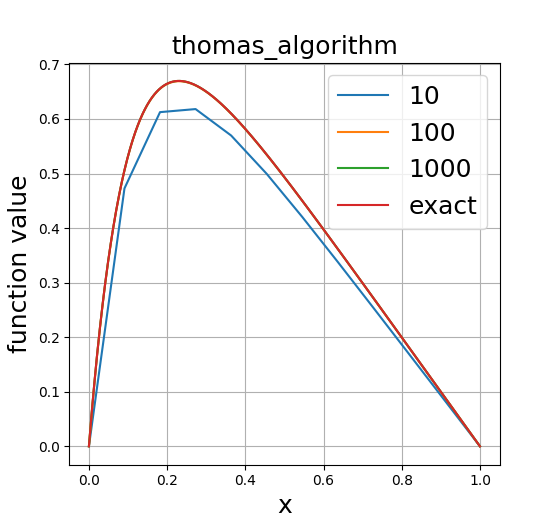
\includegraphics[scale=0.6]{thomas_data.png}
            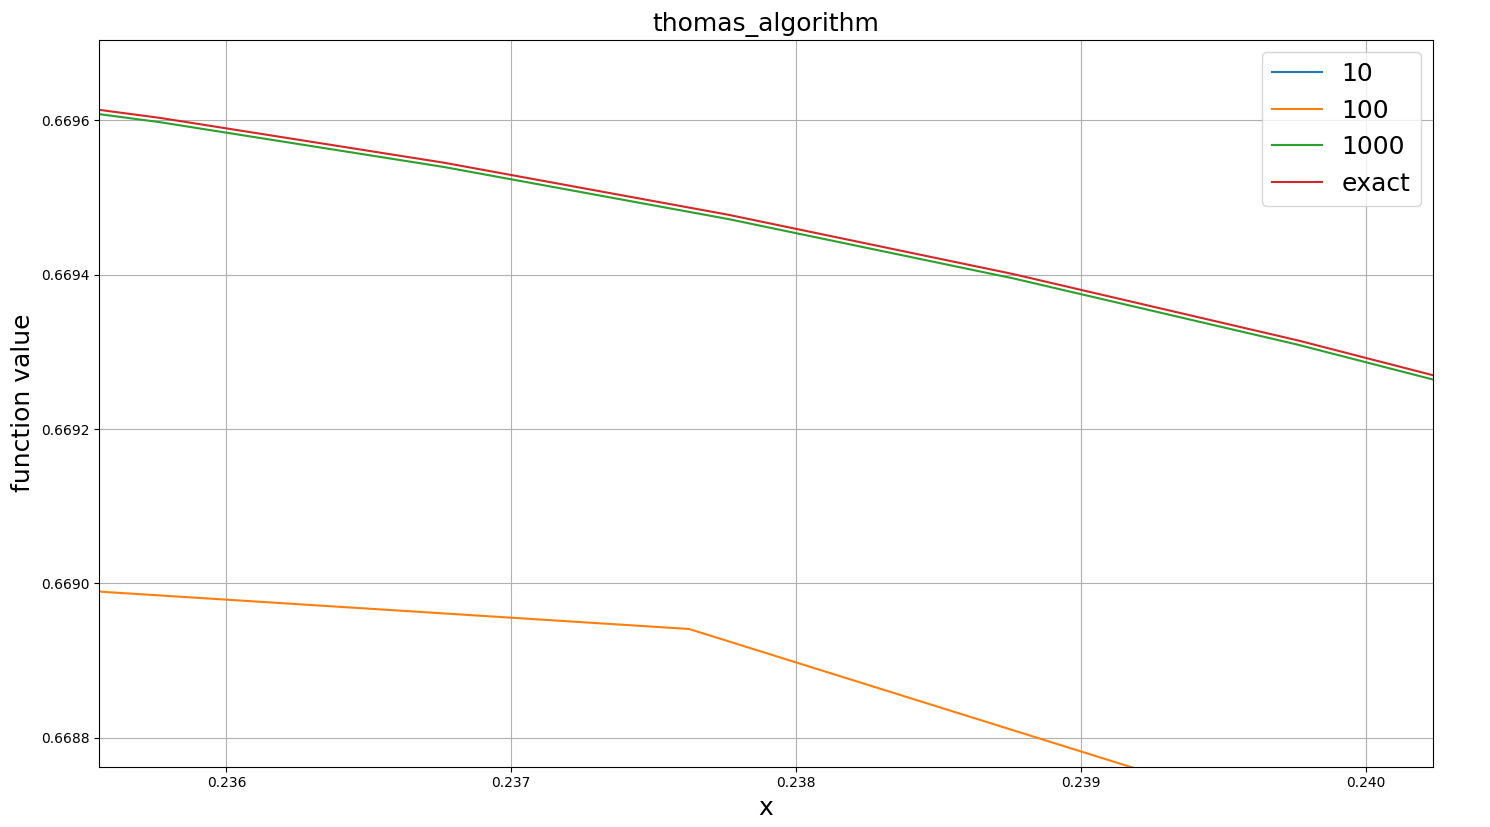
\includegraphics[scale=0.25]{thomas_data_zoom.png}
            \caption{Upper: The Thomas algorithm applied for 10, 100 and 1000 grid points on the interval \(x \in [0, 1]\). The exact value is also plotted. Lower: The same data plotted, but zoomed in to see the that the lines lie close together.}
            \label{fig:thomas_data}
        \end{figure}
        
        Figure \ref{fig:thomas_data} show how the Thomas algorithm quickly converges to the exact solution. We have chosen to not include the result for the specialized Thomas algorithm and LU decomposition, due to the fact that they look identical. This is hardly surprising, given that the three algorithms are solving the same matrix equation, only differing by the number of floating point operation needed per iteration. The only difference that could occur would be if the computer representation of the numbers is somehow different for the different algorithms. Our results show that the difference is not noticeable in our plots.
        
        The top figure shows the solution for 10, 100, and 1000 grid points along with the exact solution. The bottom figure shows a zoomed in version where we can see that for 100 grid points the computed value is very close to the exact, but the line for 1000 grid points is even more precise. As \(n\) increases, the step size gets smaller since it is defined \(h = 1/n\). A smaller step size yields higher precision as we can see in figure  \ref{fig:thomas_data}. Higher values of \(n\) converges to the exact value which is in agreement with the definition of the derivative where the step length goes to zero.
        

        
        \begin{figure}[t]
            \centering
            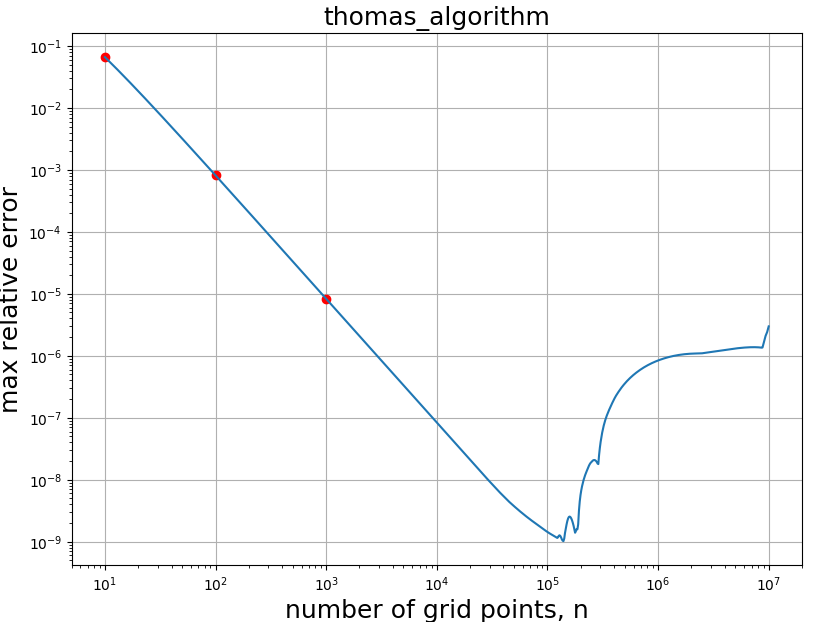
\includegraphics[scale=0.38]{error_data.png}
            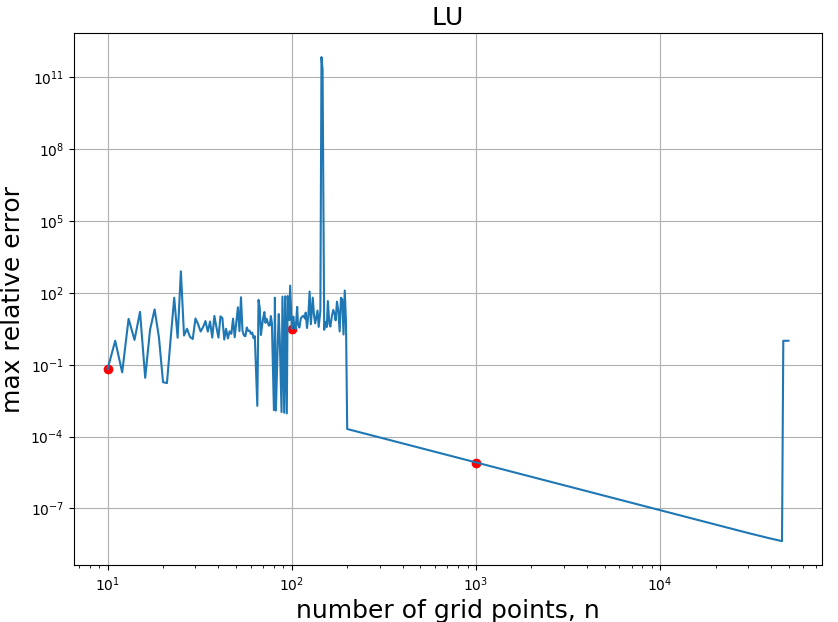
\includegraphics[scale=0.38]{error_data_LU.png}
            \caption{Upper: The figure shows how the algorithm increases linearly in precision in a log-log plot. The slope is approximately 2. After a given number of grid points (here approximately \(n=10^{5}\), the numerical error increases and takes over the analytical error. The same plot for the specialized Thomas algorithm gives the same result and is therefore not included. Lower: The maximum relative error for the LU decomposition. Due to unknown numerical problems we got unexplained values in the interval $n \approx 10$ to $n \approx 200$. Though, the rest of the graph indicates a linear decrease in relative error. The red dots indicates the relative error for $n=10$, $n=100$, $n=1000$.}
            \label{fig:error_data}
        \end{figure}

    \subsection{Error analysis}
    
        Figure \ref{fig:error_data} shows the maximum relative error from equation (\ref{eq:max_rel_error}) for the Thomas algorithm and the LU decomposition in a log-log plot. The error plot for the specialized Thomas algorithm is not included since it looks exactly like the plot for the Thomas algorithm. We see that the error in the Thomas algorithm follows a straight line, with approximately a slope of 2, until it reaches \(n=10^{5}\) where the lacking computer representation of small numbers starts to show. At this point, the numerical error increases. This follow the description we had in section \ref{sec:numerical}.%The reason for the increased relative error when \(n\) gets sufficiently large is described in section \ref{sec:numerical}.
        
        The bottom plot in figure \ref{fig:error_data} shows the LU decomposition, which displays an abnormal behaviour. We expected the error to decrease linearly, which we can see from \(n \approx 200\) to \(n \approx 14000\), but from \(n \approx 10\) to \(n \approx 200\), the max relative error varies widely. We have had a lot of cryptic error messages from armadillo's solve function on macOS for sufficiently low grid values \(n\), and we have not been able to find out why or solve the problem. The three red dots in the bottom plot of figure \ref{fig:error_data} marks where \(n = 10\), \(n=100\), and \(n=1000\). We can see that \(n=10\) and \(n=1000\) both lies on the same slope. There is also the occasional downward spike which seems to land on points on this same line. Much implies that the relative error indeed decreases linearly, and that we have an unidentified calculation error at low grid point values.
        
   

        \begin{figure}[t]
            \centering
            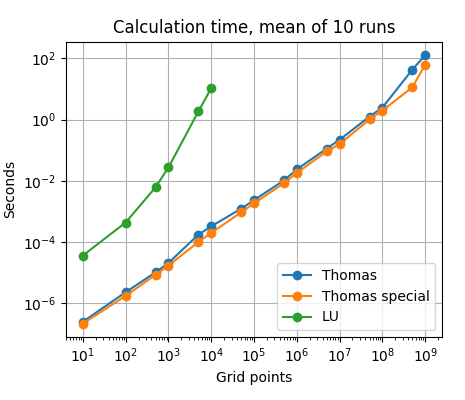
\includegraphics[scale=0.7]{algorithm_time.png}
            \caption{The figure shows the mean time usage for ten separate runs of the three different algorithms in a logarithmic plot. The LU decomposition (and the solve method from armadillo) quickly increases in time usage (as expected because of the \(2/3n^{3}\) floating point operations), and above \(10^{4}\) grid points it uses so much time that we choose to stop it there. The Thomas algorithm (and the specialized one) are fairly linear and seems to only differ in intersection point.}
            \label{fig:algorithm_time}
        \end{figure}


    \subsection{Time analysis}
        
        Figure \ref{fig:algorithm_time} show the time usage in seconds for the three different algorithms in a log-log plot. We can see that the two Thomas algorithms follow the same slope but with a constant factor separating them. This separation is due to the $4n$ and $9n$ floating point operations for the two algorithms. They differ only by a factor.
        
        What came to light pretty fast is that the LU decomposition is way too demanding to run anything as high as \(10^5\) grid points. With a grid size of \(10^5 \cdot 10^5\) we get a matrix with \(10^{10}\) grid points. If each grid point holds an integer value of 16 bits, we need approximately 20GB of memory to store the matrix. If the computer does not have this much RAM, it will start storing the data in the swap file, which will slow down the computation significantly.
        
        When we generated the numbers for the error analysis, we ran all the algorithms up to 50000 grid point values, and at that point LU used an excess of 40GB of memory. Due to the limit of our hardware at 16GB of RAM, most of the LU data was stored in swap memory, and the calculation time was very high. Over 50000 points we excluded LU and ran the two Thomas algorithms up to $10^7$ grid points. LU used approximately five hours at calculating 468 grid values, $n$, in the interval $n \in [10, 49773]$ given by $n = 10^{7i/1000}, i \in [145, 671]$. The remaining grid point values $n \in [50582, 10^7]$ were done by the Thomas algorithms in under two minutes.
            


%%%%%%%%%%%%%%%%%%%%%%%%%%%%%%%%%%%%
%%%%%%%%%%%%%%%%%%%%%%%%%%%%%%%%%%%%
\section{Conclusion}
%%%%%%%%%%%%%%%%%%%%%%%%%%%%%%%%%%%%
%%%%%%%%%%%%%%%%%%%%%%%%%%%%%%%%%%%%
    We wanted to see how we can use our knowledge in linear algebra to solve differential equations, such as Poisson's equation. We have done this by expressing the double derivative as a Taylor series. Thus we can find an expression for the analytical error. In our analysis we found out that the analytical error is proportional to $h^2$. By discretizing Poisson's equation, represented with the Taylor expansion, we constructed a matrix equation. We used three algorithms: The Thomas algorithm, a specialized Thomas algorithm, and LU decomposition followed by Gaussian elimination. The example we studied showed that we can save a lot of computation time by creating a specialized algorithm for our purpose. 

    It is apparent that LU decomposition and row reduction is a much more resource demanding way of solving a tridiagonal matrix than a tailored algorithm like the Thomas algorithm. Both memory usage and floating point operations are drastically reduced with a specialized algorithm. At large grid point values the LU decomposition is too resource hungry to be a serious tool, and at sufficiently large values impossible for most computers to use. The computer algorithms used in this report shows that the Thomas algorithm and the specialized Thomas algorithm uses $9n$ and $4n$ floating point operations respectively, compared to the $2/3n^3$ floating point operations for LU decomposition \cite[Chapter 2]{linalg}. This results in LU having a much greater computation time than the Thomas' algorithms, and the difference only becomes greater 
    
    Computers have a finite amount of storage, and therefore finite precision when it comes to storing numbers. When doing calculations like differentiation and integration, a small step size is critical for adequate precision, but at seen here a lower step size does not always mean greater precision. In our program we use double floats in C++ which according to our results and figure \ref{fig:error_data} gives a maximum precision at step lengths of approximately $10^{-5}$. Anything below will result in an increased maximum relative error. By reserving more bits per matrix element, we can increase the precision even further since the increased amount of bits allows for greater precision per number.
    
    All code used to generate data in this report is supplied in a GitHub repository at \url{https://github.com/johanafl/FYS3150-4150/tree/master/project1}.
    
    
    
    
    
    







% BIBLIOGRAPHY
\bibliography{referanser}
\bibliographystyle{aasjournal}
%\bibliographystyle{plain}

\end{document}
% Trenger referanser på poisson likning, dirichlet grensebetingelser, taylor-rekker (kap. 11 i kalkulus) og feilen fra taylor-tilnærming (kap. 9 i Knut Mørkens kompendium). Thomas algo og LU + flops til begge.

% kanskje for dirichlet boundary condition (?): https://www.researchgate.net/publication/222641921_Heritage_and_early_history_of_the_boundary_element_method